\section{Pesquisa Operacional}\label{Pesquisa Operacional}
Segundo \citeonline{depesquisa},``O início da PO (Pesquisa Operacional) teve seu surgimento na Segunda Guerra Mundial, pois os países aliados se viram confrontados com grandes problemas de logística, tática e estratégia militar. Devido à complexidade dos problemas a serem resolvidos, foram criados grupos multidisciplinares de pesquisa com objetivo de solucioná-los. O maior problema estava relacionado à utilização mais eficaz de recursos militares escassos''.

\citeonline{belfiore2012pesquisa} afirmam que ``A PO consiste na utilização de métodos científicos (modelos matemáticos e algoritmos computacionais) para a tomada de decisão''. Assim, ela utiliza esses métodos para aplicá-los a uma quantidade específica de dados e obter uma solução ótima para um problema, respeitando suas restrições. Por outro lado, \citeonline{hillier2013introduccao} destacam que   ''uma característica da PO tenta, frequentemente, encontrar uma melhor solução (conhecida como solução ótima) para o modelo que representa o problema considerado. (Diz uma melhor solução em vez de a melhor solução, pois pode haver várias soluções, cada uma delas sendo considerada como a melhor)''. Desta maneira, a PO analisa não apenas a melhoria de um ponto específico em uma empresa, mas sim todos os elementos que compõem este ponto de modo a encontrar uma solução ótima global e não pontual.

A PO está presente em várias áreas, muitas vezes dando suporte a diversas problemáticas, como por exemplo \citeonline{toso2014effective}, \emph{``Effective location models for sorting recyclables in public management''}, em que ocorre a aplicação da PO para localização de facilidade de coleta de lixo sólido urbano envolvendo LR.

\section{Logística, LRe Cadeias de Suprimentos de Circuito Fechado}\label{Logística, LRe Cadeias de Suprimentos de Circuito Fechado}

\subsection{Conceitos de Logística}\label{Conceitos Fundamentais de Logística}

Os estudos sobre a Logística, de acordo com \citeonline{buller2012logistica}, ``tiveram origem no meio militar, muito embora sua utilização remonte às mais antigas épocas na história e na economia agrária''. Os primeiros registros deste termo tiveram origem na Segunda Guerra Mundial.

A Segunda Guerra Mundial – um conflito que se originou no final da década de 30 – representou um marco significativo para o estudo da logística, pois foi durante esse período que a logística emergiu como uma ciência, uma vez que a guerra exigia não apenas ações rápidas, mas também o fornecimento de suprimentos no local apropriado e no momento certo \cite{paura2016fundamentos}.

\begin{citacao}
\textit{ Hoje, com o mercado consumidor em alta, os consumidores esperam ter grande disponibilidade de produtos para consumo. Basicamente a existência do estudo logístico existe para manter o consumidor final sempre abastecido, para que isto ocorra existe uma grande quantidade de atividades econômicas responsáveis por manter o abastecimento satisfatório tanto de produtos como de serviços. Estas atividades podem ser transporte, distribuição, aprovisionamento, gestão de materiais entre outras, para todas estas atividades em conjunto, se utiliza o termo logística \cite{costa2010logistica}}.
\end{citacao}

\subsection{Conceitos de Logística Reversa}\label{Conceitos Fundamentais de Logística Reversa}
 LRé responsável pelo processo inverso de abastecimento, ou seja, pelo retorno do produto do consumidor ao Centro de Distribuição.

\begin{citacao}
\textit{LR pode ser classificada como sendo apenas uma versão contrária da Logística como a conhecemos. O fato é que um planejamento reverso utiliza os mesmos processos que um planejamento convencional. Ambos tratam de nível de serviço, armazenagem, transporte, nível de estoque, fluxo de materiais e sistema de informação. No entanto a LR deve ser vista como um novo recurso para a lucratividade \cite{mueller2005logistica}}.
\end{citacao}

A adoção da LR por organizações tem crescido significativamente, motivada por fatores como a busca por vantagem competitiva, o aumento das preocupações ambientais e a necessidade de conformidade legal. Neste contexto, \citeonline{AGRAWAL201576} definem a LR como o processo responsável pelo planejamento, implementação e controle eficiente do fluxo de produtos, desde o ponto final de consumo até sua origem, visando a captação e recuperação de valor dos itens, seja por meio da reutilização, seja pelo descarte ambientalmente adequado. 

Embora a LR esteja em crescimento, é perceptivo a baixa exploração sobre o assunto quando relacionado a FLP, PO, PLIM, etc. De acordo com \citeonline{GOVINDAN2017371}, grande parte das pesquisas nesta área são de natureza qualitativa e setorial, sem foco quantitativo.

Em países em desenvolvimento, principalmente para as industrias, a LR tem se tornado um componente estratégico para a sustentabilidade corporativa. Seguindo esse contexto, \citeonline{MANGLA2016608} destacam a competitividade global e o apoio governamental como potencializadores da adoção da prática da LR.

\subsection{A Cadeia de Suprimentos de Circuito Fechado (CSCF)}\label{A CSCF}

A CSCF refere-se à gestão integrada dos fluxos de produtos, informações e recursos financeiros ao longo de toda a cadeia. Ela incorpora os princípios da logística direta e da logística reversa, formando assim um sistema cíclico — o chamado "circuito fechado". Conforme \citeonline{KLEINDORFER2005482}, em uma CSCF, o produto que passa por um processo oriundo de um fluxo reverso retorna ao fluxo direto, completando seu ciclo de vida por meio de um fluxo contínuo e cíclico.

A CSCF é composta por dois fluxos principais: o fluxo direto e o fluxo reverso (\autoref{fig_cscf}).

\begin{itemize}
    \item \textbf{Fluxo direto:} inicia-se com a produção das embalagens, segue para a fabricação do produto, avança até os varejistas, que disponibilizam os itens aos clientes, culminando no descarte do material após o consumo.
    \item \textbf{Fluxo reverso:} tem início no descarte realizado pelos consumidores, passando pela coleta seletiva, pelos sucateiros e, finalmente, pelo processo de reciclagem, fechando o ciclo de reaproveitamento dos materiais.
\end{itemize}

\begin{figure}[htb]
	\caption{Cadeia de Suprimento de Circuito Fechado}\label{fig_cscf}
	\begin{center}
        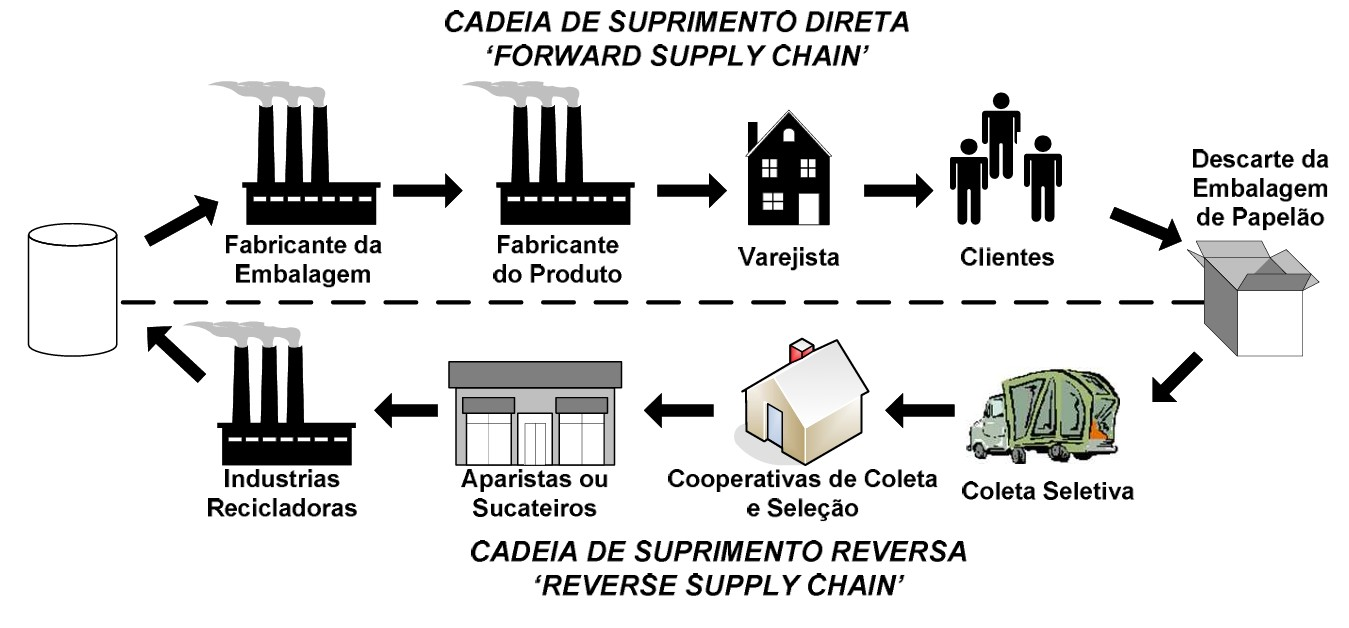
\includegraphics[width=15cm]{images/RF_img/Figura_CSCF.jpg}
	\end{center}
	\fdireta[p. 3]{Georges2009Cadeia}
\end{figure}

Neste caso foi utilizado como exemplo uma cadeia de suprimentos de embalagens, porém pode mudar algumas localidades conforme o tipo de negócio, mas o que não muda é o modelo.

Para \citeonline{GOVINDAN2015603}, devido a fatores ambientais, legais, sociais e econômicos, a CSCF passou a despertar grande interesse tanto na academia quanto no setor empresarial. Isso ocorre porque ela atua como um elemento integrador entre a logística direta e a logística reversa, sendo essencial para a recuperação de valor dos produtos e para o cumprimento de metas relacionadas à sustentabilidade.

A modelagem da CSCF é aplicável a diversos tipos de produtos, o que demonstra a versatilidade do modelo para diferentes contextos logísticos. Sua aplicação varia entre aqueles com a necessidade de um reuso rápido e constante, como o caso estudado por \citeonline{Avoleta2013Dimensionamento} sobre o dimensionamento de estoque de embalagens retornáveis. Em contraste, a CSCF também é pertinente para \textbf{bens duráveis} de longo ciclo de vida, como demonstrado na análise de \citeonline{Pereira2016Previsao} sobre a previsão de retorno de pneus inservíveis.

A CSCF, embora sua origem não esteja exclusivamente ligada a imperativos ambientais, demonstrou ser uma aliada estratégica fundamental. Ao integrar os fluxos da logística direta e da logística reversa, a CSCF permite a recuperação e valorização de materiais pós-consumo, gerando uma significativa vantagem competitiva para as empresas.

Essa evolução na gestão da cadeia converge diretamente com o conceito de \sigla{TBL}{Triple Bottom Line}, conhecido como o Tripé da Sustentabilidade. O TBL, conforme estabelecido por \citeonline{elkington1997triple}, representa a necessidade de gerenciar de forma integrada as três dimensões de desempenho: social (\emph{People}), ambiental (\emph{Planet}) e econômica (\emph{Profit}), de modo que a gestão do negócio não se restrinja à obtenção de lucros.

\subsection{A CSCF para Resíduos de Equipamentos Eletrônicos.}\label{A CSCF para Resíduos de Equipamentos Eletrônicos.}

Os motivos para a implementação da CSCF para REEE não é apenas o ambiental, além deste existe a motivação econômica e regulatória. Para, \citeonline{brito2002reverse} os motivos para investir em uma LR, e por consequência construir uma CSCF, são formadores do "triângulo de fatores" compostos pelos eixos:

\begin{itemize} 
    \item Econômico: engloba os benefícios obtidos por meio da reutilização e reciclagem de materiais, da recuperação de componentes de valor e de ganhos indiretos, como o fortalecimento da imagem da empresa por meio do marketing sustentável e a proteção estratégica, que impede o acesso de concorrentes a tecnologias ou processos produtivos próprios.
    \item Legislativo: refere-se ao conjunto de normas e obrigatoriedades a serem seguidas para redução de emissão de poluentes no meio ambiente. No contexto brasileiro, destaca-se a Política Nacional de Resíduos Sólidos, instituída pela Lei n\textordmasculine~12.305/2010 \cite{Lei12305_2010} e regulamentada pelo Decreto n\textordmasculine~10.936/2022 \cite{Decreto10936_2022}, que obriga as organizações a adotarem práticas sustentáveis ao longo de toda a sua cadeia produtiva.
    \item Responsabilidade Estendida: refere-se aos princípios éticos e de sustentabilidade que orientam as empresas a se engajarem efetivamente no desenvolvimento sustentável e na redução de impactos ambientais.    
\end{itemize}

\begin{figure}[htb]
	\caption{Triângulo de fatores.}\label{fig_tr_fat}
	\begin{center}
        \includegraphics[width=10cm]{images/RF_img/Triangulo_de_Fatores.png}
	\end{center}
	\fdireta[p. 7]{brito2002reverse}
\end{figure}

Outro ponto relevante ao tratar dos REEE diz respeito às suas características de deterioração dos itens. Muitos desses equipamentos, como telefones móveis, possuem vida útil relativamente curta, pois grande parte dos usuários utilizam por apenas dois anos. Além disso, destaca-se a possibilidade de reparabilidade, que permite o conserto e o reaproveitamento de componentes, prolongando a utilização dos produtos. Por fim, há a obsolescência programada é a limitação artificial da durabilidade dos bens manufaturados, com o intuito de incentivar o consumo repetido \cite{YlaMella2022EndofUse}.

Considerando as características de deterioração, a CSCF aplicada aos REEE envolve algumas etapas fundamentais. A primeira é a coleta, que consiste na remoção dos itens junto aos clientes, pontos de coleta, lojas e outros locais de descarte. Em seguida, ocorre a triagem, etapa em que os produtos são desmontados, separados, compactados, armazenados ou avaliados quanto ao potencial de reutilização. A fase de reprocessamento corresponde à transformação dos materiais em insumos que possam ser novamente utilizados. Por fim, ocorre a reinserção, que envolve a recomercialização do item ou do subproduto obtido por meio da reciclagem, reintegrando-o ao ciclo produtivo \cite[apud Mendes, 2017]{pereira2018logistica}.

\section{Problemas de Localização de Facilidades na Cadeia Logística}\label{Problemas de localização e alocação de facilidades na cadeia logística}
Problemas de localização e alocação de facilidades é uma das linhas de pesquisa que se desenvolvem metodologias na área logística, pode-se verificar a grande importância do assunto quando se verifica o caso da empresa \emph{Leaseway Transportation Corporation}, em que foi utilizado a metodologia de Localização de Alocação de Facilidades conhecida como Centro de Gravidade. Com esta aplicação a companhia conseguiu definir a localização de uma instalação de manutenção de caminhões em Boston \cite{ballou2006gerenciamento}.

Segundo \citeonline{arakaki2006heuristica}, a FLP é um aspecto crítico no planejamento estratégico para um grande espectro de empresas públicas e privadas. Seja um empresário que quer construir um novo shopping, um industrial que deseja situar uma nova fábrica ou um administrador público que quer estabelecer postos de saúde, são frequentemente desafiados pela dificuldade de decidir por um local adequado, com isso percebe-se o grande valor que possui este tipo de estudo, podendo se tornar um diferencial competitivo.

Muitas vezes, este estudo deve contar com a Pesquisa Operacional (PO) como suporte para os cálculos necessários a fim de encontrar a melhor solução possível, ou com a função objetivo (FO). Um exemplo disso é o estudo de \citeonline{medrano2020using}, que define um problema de localização de máxima cobertura para a LR de produtos no fim do ciclo de vida, onde a PO foi utilizada para a execução das análises. Além disso, é importante ressaltar que a LR também fará parte desta dissertação de mestrado.

Para gestão de resíduos e recuperação de materiais, o planejamento de FLP é de grande criticidade, pois a definição de quantidade de facilidades e suas localizações possuem um impacto enorme na eficiência de transportes, \citeonline{TOSO2014839} demonstram a possibilidade da aplicação de dois modelos, um determinístico e um estocástico para se obter uma solução ótima.

\section{Programação Linear Inteira Mista (PLIM)}

A técnica de PLIM caracteriza-se pela presença simultânea de variáveis de decisão contínuas e discretas. As variáveis contínuas podem representar, por exemplo, a quantidade de movimentações de itens ou o nível de estoque em um CSCF, enquanto as variáveis discretas estão associadas à ativação de localidades, modeladas por meio de variáveis binárias. Segundo \citeonline{Camelo2024}, o PLIM se destaca por fornecer ferramentas para o planejamento logístico, integrando de maneira eficiente decisões estratégicas e operacionais em cadeias de suprimentos complexas voltadas para o hidrogênio verde.

Por se tratar de uma abordagem de PO, a modelagem por PLIM envolve três componentes fundamentais: a função objetivo, que define o propósito da otimização — podendo ser de maximização ou minimização; as variáveis de decisão, determinadas pela formulação computacional do modelo, que podem ser contínuas, inteiras ou binárias; e os conjuntos de restrições, que representam limitações como capacidades, regras de negócio, localizações pré-definidas, entre outras. Essa estrutura é exemplificada em \citeonline{Guzman2023Matheuristic}, que propõem um modelo de PLIM voltado à minimização dos custos de produção, estoque, transporte e atraso. O modelo considera variáveis de decisão como nível de estoque, quantidade de produtos transportados e produzidos, e ativação de plantas industriais, utilizando parâmetros como custos unitários de transporte, produção e armazenagem, demanda, capacidades máximas de estoque e custo de abertura.

A PLIM é amplamente empregada em modelos de localização de CDs e PAs, bem como no dimensionamento de estoques em CSCF. Segundo \citeonline{Vicente2025}, que aplica a PLIM na revisão periódica de estoques de uma cadeia de suprimentos com múltiplos estágios, os resultados obtidos indicam melhorias significativas na configuração da rede e redução expressiva de custos operacionais de pedido, transportes e manutenção.

Neste trabalho, ao abordar a CSCF de adquirência, que inclui a presença de CDs, PAs, além de fluxos diretos e reversos, a representação do problema por meio de um modelo PLIM é escolhida, pois permite modelar tanto variáveis binárias quanto variáveis contínuas, tudo inserido no contexto de uma função objetivo de minimização do custo total. Estudos recentes corroboram com esta escolha como é o caso de \citeonline{Oujana2023} que utilizam a mesma abordagem  para resolução de sistemas complexos de agendamento de produção, distribuição e estoques de uma planta de embalagens.